\section{Birth-plague model}

Birth
$$\pr{\Delta \xt = 1, \Delta \yt = 0} = \beta \xt \Delta t +o(\Delta t)$$
Corruption (instantiation of plague)
$$\pr{\Delta \xt = -1, \Delta \yt = 1} = \delta \xt \Delta t +o(\Delta t)$$
Infection (spreading of plague)
$$\pr{\Delta \xt = -1, \Delta \yt = 1} = \alpha \xt\yt \Delta t +o(\Delta t)$$
Dying (death of plague infected)
$$\pr{\Delta \xt = 0, \Delta \yt = -1} = \mu \yt \Delta t +o(\Delta t)$$
No event
$$\pr{\Delta \xt = \Delta \yt = 0} =1 - \lrbs{(\beta + \delta + \alpha \yt) \xt + \mu \yt} \Delta t +o(\Delta t)$$



\begin{figure}[h!]
    \centering
    % First row
    \begin{subfigure}{0.49\textwidth}
        \centering
        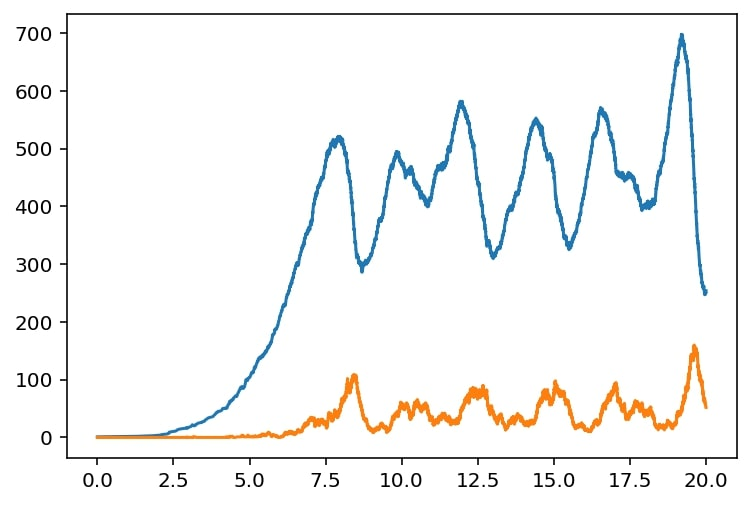
\includegraphics[width=\linewidth]{figures/root/bpPLOT}
        \label{fig:figure1}
    \end{subfigure}
    \hfill
    \begin{subfigure}{0.49\textwidth}
        \centering
        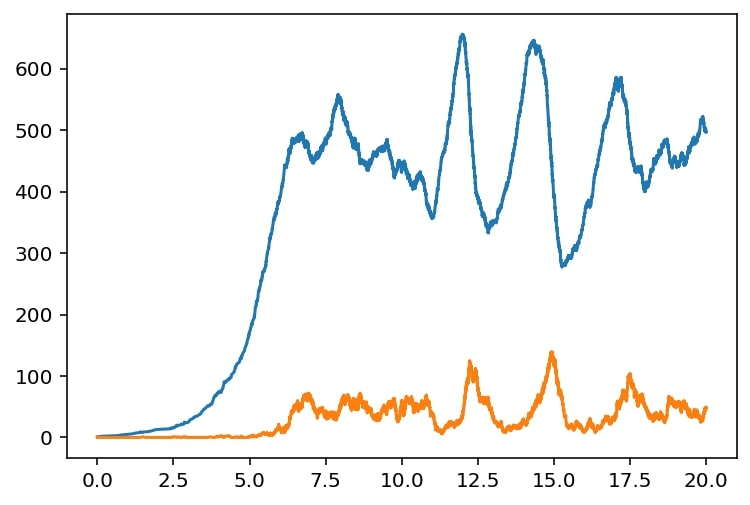
\includegraphics[width=\linewidth]{figures/root/bpPLOT2}
        \label{fig:figure2}
    \end{subfigure}
    
    % Second row
    \vspace{0.5cm} % Optional: adds some space between rows
    \begin{subfigure}{0.49\textwidth}
        \centering
        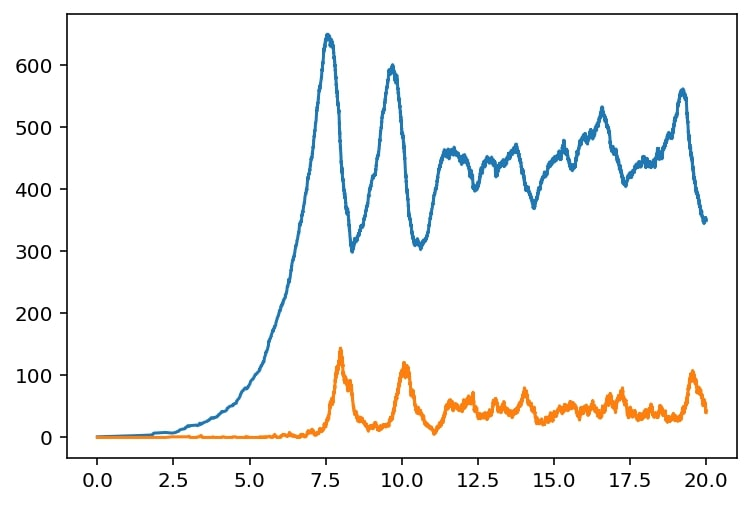
\includegraphics[width=\linewidth]{figures/root/bpPLOT3}
        \label{fig:figure3}
    \end{subfigure}
    \hfill
    \begin{subfigure}{0.49\textwidth}
        \centering
        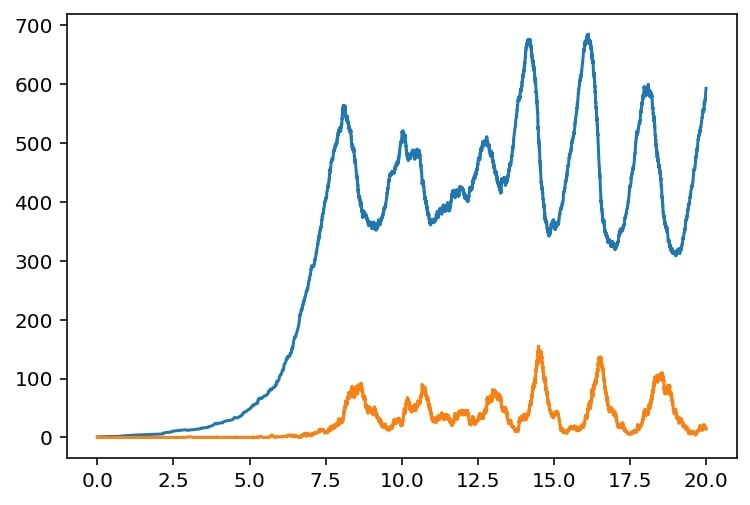
\includegraphics[width=\linewidth]{figures/root/bpPLOT4}
        \label{fig:figure4}
    \end{subfigure}
    
    \caption{($\beta, \delta, \alpha, \mu$) = (birth, corruption, infection , dying) = (1, 0.1, 0.02, 10). Four realisations of the birth plague model. In each, the blue line is $\xt$ (population count), $\yt$ is the number of plague infected individuals.}
    \label{fig:four-figures}
\end{figure}
